

\documentclass[a4paper, 11pt, english, fleqn]{article}
\usepackage[utf8]{inputenc}
\usepackage{babel}
%\usepackage{ngerman}
\usepackage{coordsys,logsys,color}
\usepackage{fancyhdr}
\usepackage{hyperref}
\usepackage{texdraw}				
\usepackage[T1]{fontenc}					
\usepackage{amsmath,amsfonts,amssymb}	
\usepackage[normalem]{ulem}	
\usepackage{listings}
\usepackage{graphicx}
\usepackage{enumitem}
\usepackage[paper=a4paper,left=35mm,right=35mm,top=35mm,bottom=30mm]{geometry}

\hypersetup{colorlinks=true, breaklinks=true, linkcolor=darkblue, menucolor=black, urlcolor=darkblue, citecolor=darkblue}

\pagestyle{fancy}

\renewcommand{\familydefault}{cmss}

\definecolor{fgcgray}{rgb}{0.4, 0.4, 0.4}
\definecolor{darkblue}{rgb}{0,0, 0.4}
\newcommand{\titlefont}[1]{\textcolor{black}{\fontseries{bx}\fontshape{n}\fontsize{30}{0pt} \selectfont #1}}
\newcommand{\titlepagef}[1]{\textcolor{black}{\fontseries{bx}\fontshape{n}\fontsize{14}{0pt} \selectfont #1}}

\newcommand{\gloss}[1]{\textcolor{glossb}{\fontsize{11}{0pt}\selectfont #1}}

\newlist{aims}{enumerate}{1}
\setlist[aims,1]{
	label={Aim~\arabic*},
	leftmargin=*,
	align=left,
	%labelsep=1mm,
	font=\bfseries
}

\addtolength{\oddsidemargin}{-1.0cm}
\addtolength{\evensidemargin}{-1.0cm}
\addtolength{\headwidth}{2.0cm}
\addtolength{\textwidth}{2.0cm}

\setlength{\parindent}{0cm}

\renewcommand{\labelitemi}{$\circ$}
\renewcommand{\labelitemii}{$\diamond$}

\newcommand{\spaceline}[1][8pt]{\vskip #1}
\newcommand{\attrname}[1]{\textcolor{fgcgray}{\scriptsize #1}}

\newcommand{\comment}[1]{\spaceline[5pt] \textcolor{fgcgray}{\scriptsize #1} \spaceline[15pt]}

\makeatletter

\newcommand*{\project}[1]{\gdef\@project{#1}}


\def\@maketitle{
  %\begin{titlepage}
   
  \begin{center}
      \titlepagef{Software-Project 2017}
      \spaceline
  \end{center}
  
  \begin{center}
      \parbox{\textwidth}{
        \spaceline
        \centering{\titlefont{Detailed Design}}
        \par
        \spaceline
      }
  \end{center}
  
  \begin{center}
  	\titlepagef{Real-Time Mesh Utilities}
  	\spaceline[2em]
  \end{center}
  
  \begin{center}
  \begin{tabbing}
  Petros Simidyan \qquad \=
  Blerta Hamzallari \qquad \=
  Felix Griesau \qquad \=
  Marco Klamke \\
  Julius Lerm
  \>Lars Debor
  \>Simon Heinke  
  \>Sugandha Sachdeva
  \end{tabbing}
  \end{center}
 
  
  \spaceline[3em] {
    \begin{flushright}
    \begin{tabular}[t]{rl}
      \attrname{last change:} & \@date
    \end{tabular}
    \end{flushright}
    \par
  }
  \spaceline[5.5em]
  %\end{titlepage}
}

\begin{document}

\pagenumbering{gobble}
	
\lhead{\sc{Detailed Design: RTMU}}	
\title{Detailed Design: RTMU}
\vspace{3 in}
\maketitle


\includegraphics[width = \linewidth]{figures/mne-cpp.png}

\clearpage

\pagenumbering{arabic}

\tableofcontents

\clearpage
\section{General Architecture}

\subsection{GeometryInfo}

The class \textit{GeometryInfo} holds all needed functions for the Surface Constrained Distance Calculation (from now on abbreviated with SCDC) and the Sensor Projecting (see Functional Specification for further details). Since all functions are static, the class itself does not have to be instantiated, thus the class is declared static and the default constructor is forbidden.

\begin{figure}[h]
	\begin{center}
		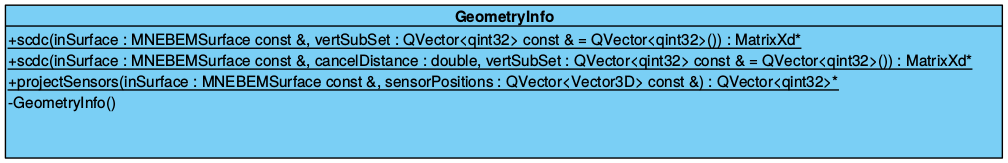
\includegraphics[width=16cm]{figures/geometryinfoclassdiagram.png}
		\caption{Interface of GeometryInfo}
	\end{center}
\end{figure}

\subsubsection{Method: \textit{scdc}}
The method @todo(oder function ?) receives bla bla bla

\subsubsection{Method: \textit{iterativeDijkstra}}
asdf

\subsubsection{Method: \textit{projectSensor}}
asdf

\subsubsection{Method: \textit{matrixDump}}
asdf

\clearpage

\section{Subdivision of Program Features}

\begin{aims}
	
	\item[SCDC] 
	The surface constrained distance calculation algorithm receives a mesh data set as its input, which is stored inside a file. It then calculates approximate distances between vertices. When no further input arguments are provided, the SCDC algorithm calculates a full distance table, i.e. the distance between any vertex to any other vertex.
	When it receives a subset of the vertices as an additional argument, it only calculates the distances from said subset to every other vertex of the mesh. The SCDC algorithm stores its results inside a two-dimensional matrix.
	
	\item[Projecting]
	The projecting algorithm maps MEG/EEG-sensors to vertices of the mesh. In case of MEG-sensors, the orientation is known and thus a radial projection is applied in order to assign each sensor to a vertex. In case of EEG-sensors, the orientation is not known and a nearest-neighbor algorithm is used.
	The projecting algorithm then outputs the results of the calculation as an array of indices, which point to the respective vertices of the mesh.
	
	\item[Interpolation]
	The interpolation algorithm uses the results of both the projecting algorithm and the SCDC algorithm.
	Based on the distance table, it calculates a weight matrix for the later live interpolation. 
	Thus the interpolation algorithm receives three different inputs: the distance table created by SCDC, the sensors mapping and the actual sensor input, i.e. brain activity recorded by sensors over a period of time.
	The recorded brain activity gets passed to the interpolation algorithm either from an ongoing MEG/EEG scan or a prerecorded data set, i.e. a file. 
	
	\item[Disp3D]
	In order to provide control over aspects of the interpolation within the MNE-CPP framework, a new function is added to the Disp3D tree model.
		
\end{aims}

By dividing the real-time mesh utilities into the mentioned components, internal changes and extensions are easy to implement. Added to that, the single components can be reused elsewhere within the MNE-CPP framework.

\clearpage

\section{Basic Structure and Interface}

\begin{aims}
	\item[GeometryInfo] To provide the highest possible level of usability and versatility, a function to calculate surface constrained distances as well as the sensor-to-mesh mapping can be found inside the class \textit{GeometryInfo}. The mentioned option to provide a subset of vertices for the SCDC can be omitted by passing an empty vector as the second argument. 

\begin{figure}[h]
	\begin{center}
		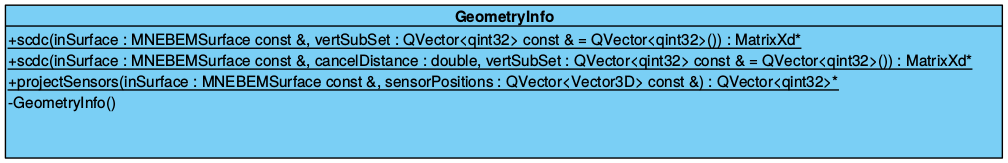
\includegraphics[width=16cm]{figures/geometryinfoclassdiagram.png}
		\caption{Interface of GeometryInfo}
	\end{center}
\end{figure}

\item[Interpolation] In order to keep the interpolation of neurophysiological activity efficient, the mentioned weight matrix (see section 2) is stored as a member of type MatrixXd inside the class \textit{Interpolation}, or rather as a pointer to such.
To use the precalculated weight matrix, one has to pass the current set of sensor data to the function \textit{interpolateSignals} and receives the results as a vector.

\begin{figure}[h]
	\begin{center}
		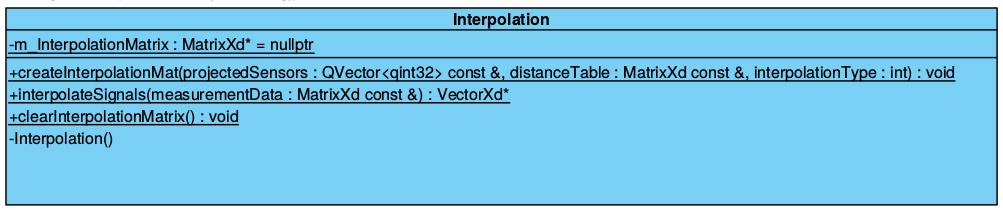
\includegraphics[width=16cm]{figures/interpolationclassdiagram.png}
		\caption{Interface of Interpolation}
	\end{center}
\end{figure}

\clearpage

\item[SensorDataTreeItem] To achieve the mentioned integration into the GUI framework, the program must integrate the SensorDataTreeItem.

\begin{figure}[h]
	\begin{center}
		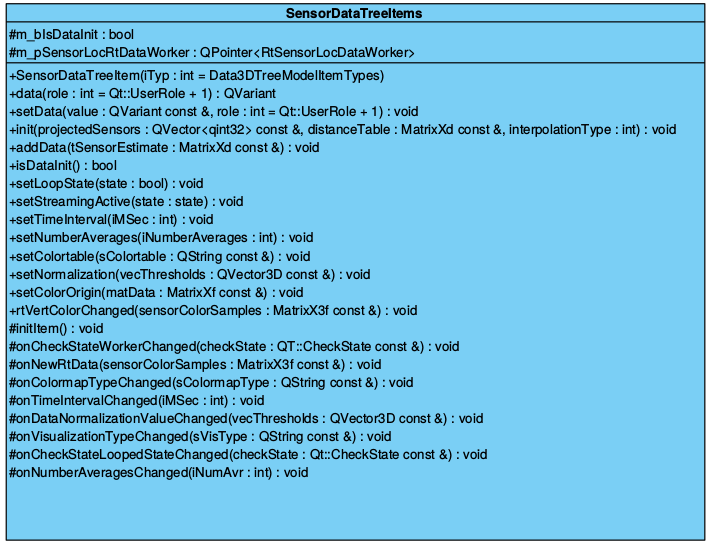
\includegraphics[width=16cm]{figures/sensordatatreeitemclassdiagram.png}
		\caption{SensorDataTreeItem}
	\end{center}
\end{figure}

\end{aims}

\begin{figure}[h]
	\begin{center}
		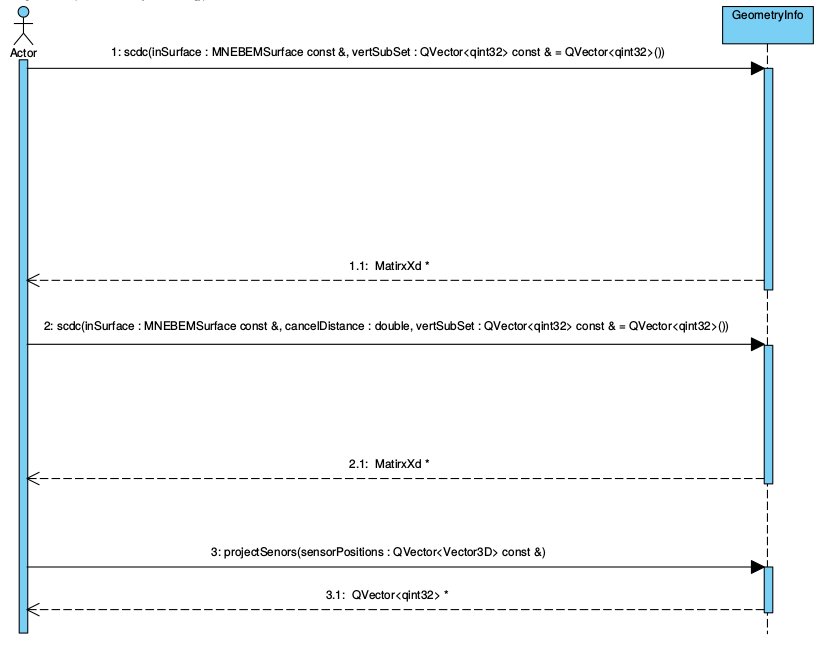
\includegraphics[width=16cm]{figures/geometryinfo_calling_sequence.png}
		\caption{Geometry calling sequence}
	\end{center}
\end{figure}

\begin{figure}[h]
	\begin{center}
		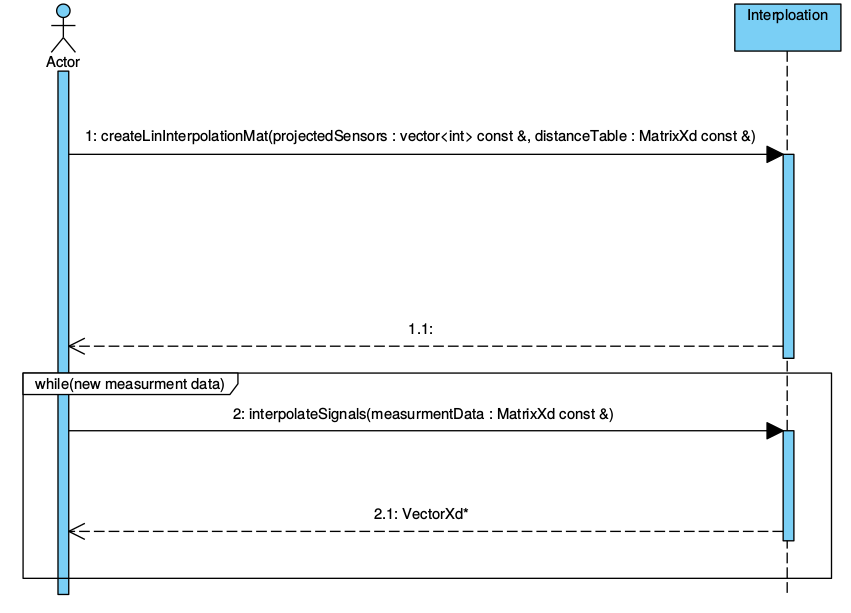
\includegraphics[width=16cm]{figures/interpolation_calling_sequence.png}
		\caption{Interpolation calling sequence}
	\end{center}
\end{figure}

\clearpage
  
\end{document}
